mybot111222\documentclass[10pt]{beamer}

\usetheme{CambridgeUS}
\usepackage[english, russian]{babel}
\usepackage[utf8]{inputenc}
\usepackage{caption}
\usepackage{etoolbox}
\usepackage{multicol}
\usepackage{listings}
\usepackage{wasysym}
\usepackage{mathtools}
\DeclarePairedDelimiter\ceil{\lceil}{\rceil}
\DeclarePairedDelimiter\floor{\lfloor}{\rfloor}

\definecolor{mygreen}{rgb}{0,0.6,0}
\lstset{
  basicstyle=\ttfamily\footnotesize,        % the size of the fonts that are used for the code
  breaklines=true,                 % automatic line breaking only at whitespace
  captionpos=b,                    % sets the caption-position to bottom
  commentstyle=\color{mygreen},    % comment style
  keywordstyle=\color{blue},       % keyword style
  stringstyle=\color{red},     % string literal style
  showstringspaces=false,
  morekeywords={include, printf},
  texcl=true     %<---- added
}


\title[\href{https://goo.gl/NRgp8K}{https://goo.gl/NRgp8K} (Term 2)]{Lowest Common Ancestor}
\author[Гусев Илья, Булгаков Илья]{Гусев Илья, Булгаков Илья}
\institute[МФТИ] 
{Московский физико-технический институт\\*}
\date{Москва, 2019}
\subject{Computer Science}

\begin{document}

\begin{frame}
  \titlepage
\end{frame}

\begin{frame}{Содержание}
\tableofcontents
\end{frame}


\section{Небинарные деревья}

\begin{frame}[fragile]{Небинарные деревья}
Деревья бывают не только бинарные! \\
Мы раньше работали в основном с \textbf{бинарными деревьями}, но это частный случай более общего вида дерева, которое может ветвиться больше, чем на две дочки.

\begin{center}
    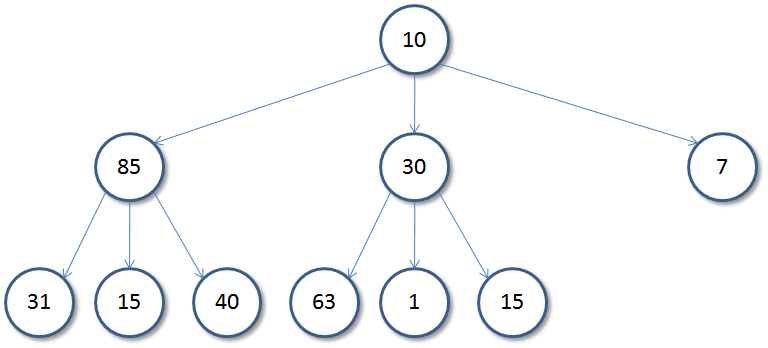
\includegraphics[height=5cm]{Term_2/Source/images/10-ternary_tree.png}
\end{center}

\end{frame}

\begin{frame}[fragile]{Как реализовать небинарное дерево?}

Два способа представления небинарных деревьев:
\begin{enumerate}
    \item Структура узла: \{data, parent, next, first\} \\
Минусы: new на узел, требуется много памяти. \\
Плюсы: удобно работать
    \item Структура узла: \{data, parent\} \\
Минусы: неудобно делать обход в глубину \\
Плюсы: хранится компактно, для некоторых задач этого достаточно (например, LCA -- об этом ниже)
\end{enumerate}

\end{frame}

\section{Задача LCA}

\begin{frame}[fragile]{Задача LCA}
LCA - Lowest (least) Common Ancestor \\ Задача нахождения наименьшего общего предка (нижайший общий предок) вершин u и v в корневом дереве T.\\

\begin{center}
    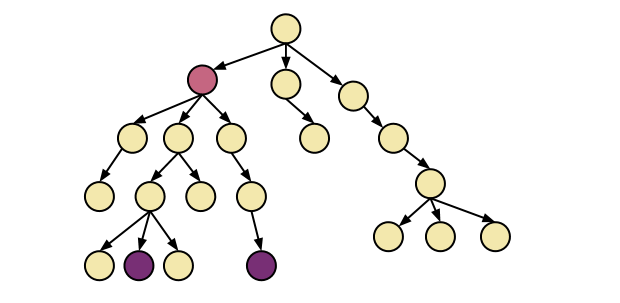
\includegraphics[height=5cm]{Term_2/Source/images/10-Finding-the-Lowest-Common-Ancestor.png}
\end{center}

\end{frame}


\begin{frame}[fragile]{LCA - тривиальное решение}
Тривиальное решение задачи LCA
\begin{lstlisting}
LCA(u, v):
    h1 := depth(u)
    h2 := depth(v)
  
    while h1 != h2:
       if h1 > h2:
          u := parent(u)
          h1 := h1 - 1
       else:
          v := parent(v)
          h2 := h2 - 1
  
    while u != v:
       u := parent(u)
       v := parent(v)
  
    return u
\end{lstlisting}
Сложность?
\end{frame}



\section{Метод двоичного подъема для LCA}

\begin{frame}[fragile]{Метод двоичного подъема для LCA}

Мотивация: решение за O(n) долгое, хотим быстрее. \\
Идея метода: выполним препроцессинг, в ходе которого вычислим предков на некоторых глубинах -- вычислим для каждой вершины её 1-го предка, 2-го предка, 4-го, 8-го.

\begin{center}
    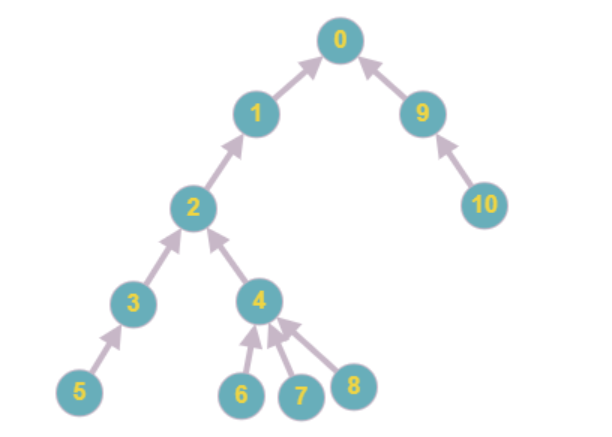
\includegraphics[height=4cm]{Term_2/Source/images/10-lca.png}
\end{center}

\end{frame}


\begin{frame}[fragile]{Метод двоичного подъема для LCA}
Что мы вычисляем в препроцессинге:
\begin{itemize}
    \item Массив предков P, т.е. $P[i][j]$ - это $2^j$-й предок вершины $i$, $i = 1..N, j = 0..⌈log N⌉$ \\
Например, \\
P[5][0] = 3 \\
P[5][1] = 2 \\ 
P[5][2] = 0 \\
\end{itemize}
\begin{center}
    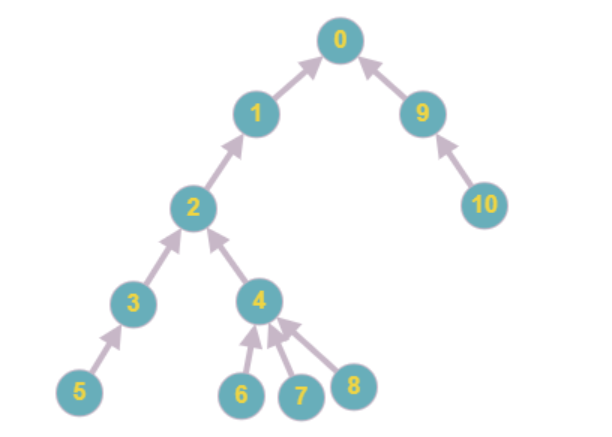
\includegraphics[height=4cm]{Term_2/Source/images/10-lca.png}
\end{center}
\end{frame}

\begin{frame}[fragile]{Метод двоичного подъема для LCA}
Что мы вычисляем в препроцессинге:
\begin{itemize}
    \item Для каждой вершины сохраняем пометки входа и выхода при обходе в глубину. Это удобно для определения является ли одна вершина родителем другой: если интервал входа/выхода одной вложен в другой, значит, является обрамляющая является родителем.
\end{itemize}
\begin{center}
    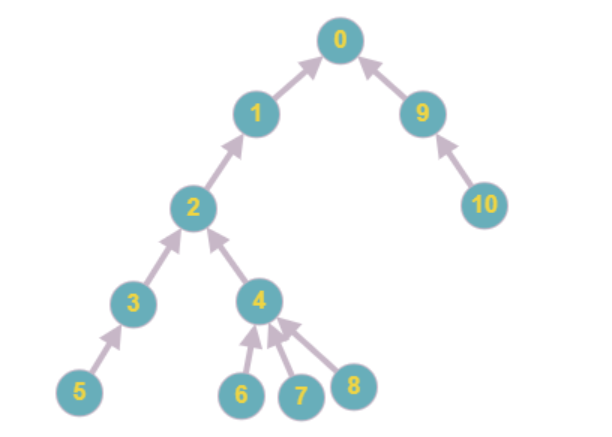
\includegraphics[height=4cm]{Term_2/Source/images/10-lca.png}
\end{center}
\end{frame}


\begin{frame}[fragile]{Метод двоичного подъема для LCA}
Как мы делаем препроцессинг?
\begin{itemize}
    \item Запускаем DFS. Вычислим для каждой вершины позицию входа и выхода в массиве входов/выходов при обходе в глубину. \\
(0 1 2 3 5 5 3 4 6 6 7 7 8 8 4 2 1 9 10 10 9 0) \\
Первое упоминание - вход, втрое - выход
    \item Удобно вычислить родителей 0 уровня, т.е. $P[i][0]$, прямо тут. 
    \item Динамикой довычисляем все уровни от 1 до log(n) \\
P[v][i] = P[P[v][i-1]][i-1]; // Подъем на i это два подъема на i-1. Подъем на 8 - это два подъема на 4.
\end{itemize}
\begin{center}
    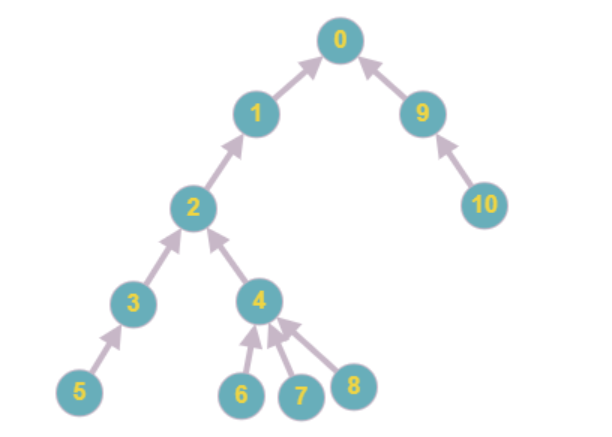
\includegraphics[height=4cm]{Term_2/Source/images/10-lca.png}
\end{center}
\end{frame}

\begin{frame}[fragile]{Метод двоичного подъема для LCA}
Как искать ответ?
\begin{itemize}
    \item Проверим, не является ли одна вершина предком другой - в таком случае она и является результатом.
    \item Будем подниматься по предкам A, пока не найдем самую высокую (т.е. наиболее близкую к корню) вершину, которая ещё не является предком (не обязательно непосредственным) B. Т.е. такую вершину X, что X не предок B, а P[X][0] - предок B. \\
    Как: пусть сначала I = ⌈log N⌉. Если P[A][I] не является предком B, то присваиваем A = P[A][I], и уменьшаем I. Если же P[A][I] является предком B, то просто уменьшаем I. Очевидно, что когда I станет меньше нуля, вершина A как раз и будет являться искомой вершиной - т.е. такой, что A не предок B, но P[A][0] - предок B.
\end{itemize}
\end{frame}

\begin{frame}[fragile]{Метод двоичного подъема для LCA}
\textbf{Пример}. Вычислим общего предка для 5, 10 \\
l = log2 (11) по числу вершин \\
A = 5, B = 10, l=4. P[A][l] == 0, 0 является предком B \\
A = 5, B = 10, l=3. P[A][l] == 0, 0 является предком B \\
A = 5, B = 10, l=2. P[A][l] == 0, 0 является предком B \\
A = 5, B = 10, l=1. P[A][l] == 2, 2 не является предком B \\
A = 2, B = 10, l=0. P[A][l] == 1, 1 не является предком B \\
A = 1, B = 10, l=-1. Останов.

\begin{center}
    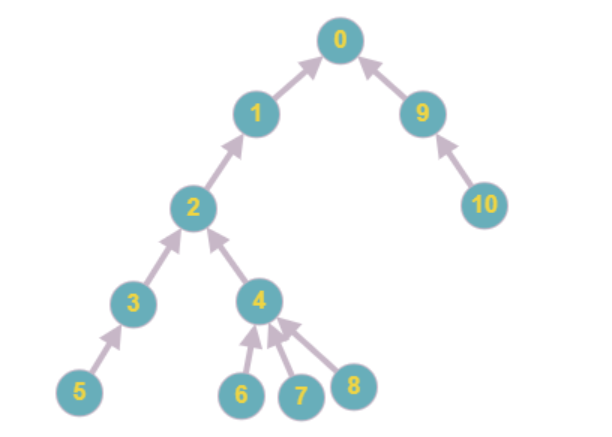
\includegraphics[height=4cm]{Term_2/Source/images/10-lca.png}
\end{center}
\end{frame}

\section{LCA $\rightarrow$ RMQ}
\begin{frame}[fragile]{LCA $\rightarrow$ RMQ}
\begin{center}
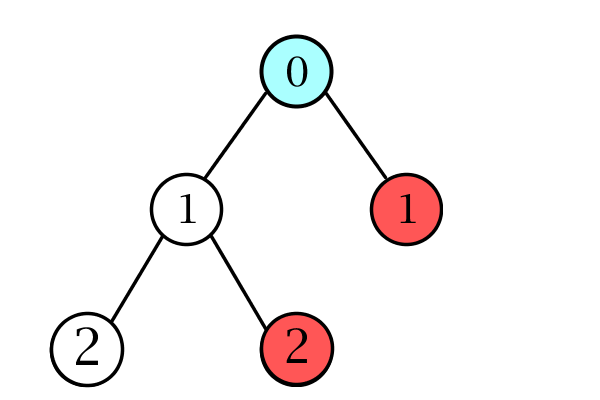
\includegraphics[height=4cm]{Term_2/Source/images/lca2rmq.png}\\
\end{center}
DFS по глубинам (d): 012121010\\
DFS по вершинам (vtx): 012131040\\
LCA(3,4) = vtx[rmq(d, I(3), I(4))] = vtx[rmq(d, 4, 7)] = vtx[argmin(2101) + 4] = vtx[6] = 0\\
\end{frame}

\section{RMQ $\rightarrow$ LCA}
\begin{frame}[fragile]{Декартово дерево по неявному ключу}
Декартово дерево - бинарное дерево поиска слева направо и куча сверху вниз\\
Неявный ключ - количество элементов в нашей структуре, находящихся левее нашего элемента\\
Эквивалентное определение:
\begin{itemize}
    \item Корнем дерева является элемент массива, имеющий минимальное значение A, скажем A[i]
    \item Левым поддеревом является декартово дерево по неявному ключу на массиве A[1..i-1]
    \item Правым поддеревом является декартово дерево по неявному ключу на массиве A[i+1..N]
\end{itemize}
\end{frame}

\begin{frame}[fragile]{RMQ $\rightarrow$ LCA}
\begin{center}
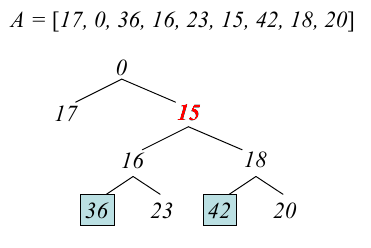
\includegraphics[height=4cm]{Term_2/Source/images/rmq2lca.png}\\
\end{center}
RMQ(i, j) = LCA(A[i], A[j])
\end{frame}

\appendix

\begin{frame}[allowframebreaks]
  \frametitle<presentation>{Полезные ссылки}
    
  \begin{thebibliography}{10}
{
  \beamertemplatebookbibitems
  % Start with overview books.

  \bibitem{emaxx}
  \texttt{E-maxx: метод двоичного подъёма}
  \newblock \href{http://e-maxx.ru/algo/lca\_simpler}
  {\texttt{http://e-maxx.ru/algo/lca\_simpler}}
  
  \bibitem{wiki1}
  \texttt{Викиконспекты: LCA2RMQ}
  \newblock \href{http://bit.ly/2vGza6e}
  {\texttt{http://bit.ly/2vGza6e}}
  
  \bibitem{wiki1}
  \texttt{Викиконспекты: RMQ2LCA}
  \newblock \href{http://bit.ly/2vDI2tp}
  {\texttt{http://bit.ly/2vDI2tp}}
}
  \end{thebibliography}
  \end{frame}

\end{document}


